\section{Анализ предметной области}
\subsection{История игр жанра платформер }
История жанра "платформер" связана с рождением видеоигр и является одной из самых долгоживущих и популярных категорий игр. Этот жанр включает в себя множество игр, где игрок управляет персонажем, перескакивая с платформы на платформу, преодолевая препятствия и собирая различные предметы. Вот краткая история развития жанра платформер:

1. 1970-е годы: Первые шаги\obeylines
Первыми играми, которые можно отнести к жанру платформер, были аркадные классики, такие как "Donkey Kong" (1981) и "Space Panic" (1980). В "Donkey Kong" игрок управлял персонажем по имени Марио, который должен был перепрыгивать через платформы, чтобы спасти принцессу от гориллы Донки Конга.

2. 1980-е годы: Золотая эра
1980-е годы стали золотой эрой для жанра. Игры, такие как "Super Mario Bros." (1985) и "Sonic the Hedgehog" (1991), стали символами этой эпохи. "Super Mario Bros." представил мир Марио, который стал одним из самых узнаваемых персонажей в истории видеоигр. Игры этого периода установили стандарты для геймплея, включая сбор монет, прыжки и бег.

3. 1990-е годы: Развитие жанра
В 1990-е годы жанр платформер продолжил развиваться. Игры, такие как "Super Mario 64" (1996) и "Crash Bandicoot" (1996), перевели жанр в 3D пространство, предоставив игрокам свободу движения и исследования.

4. 2000-е годы: Эксперименты и инновации
В начале 2000-х годов, жанр платформер стал подвергаться инновациям и экспериментам. "Portal" (2007) предложил уникальный геймплей с использованием порталов, а "Braid" (2008) внес элементы временной манипуляции в платформеры.

5. 2010-е годы: Возвращение классики
В последнее десятилетие, наблюдается возвращение к классическим платформерам. Игры, такие как "Super Meat Boy" (2010) и "Cuphead" (2017), предложили сложные вызовы и стилизацию визуального дизайна, вдохновленные играми 8-битных и 16-битных консолей.

6. Современность: Разнообразие и творчество
В настоящее время жанр платформер продолжает развиваться с новыми идеями и подходами. Инди-разработчики вносят свои инновации, создавая уникальные и непредсказуемые игры в этом жанре. 

Жанр платформер остается популярным как среди опытных игроков, так и среди новичков, благодаря простой и понятной механике игры. В течение многих десятилетий, он оставался одним из самых важных и веселых жанров в мире видеоигр.
\subsection{Игра Montezuma's Revenge }
"Montezuma's Revenge" (или "Montezuma's Revenge: Featuring Panama Joe") - это классическая видеоигра, выпущенная в 1984 году компанией Parker Brothers. Она была разработана Робертом Янгом и является одной из популярных игр для платформы Atari 8-бит и многих других игровых систем того времени.

Игра Montezuma's Revenge представляет собой платформенный приключенческий проект, где игрок управляет персонажем по имени Панама Джо. Игровой сценарий отправляет игрока в древний храм Монтесумы, где Джо должен собирать сокровища и убегать от ловушек и врагов.

Главной целью игры является проникновение в глубины храма, где находятся сокровища, и собрать как можно больше из них. Персонаж может бегать, прыгать, лазить по лестницам и использовать предметы, чтобы преодолеть преграды. В игре присутствуют различные враги и ловушки, такие как скелеты, змеи, пламя и даже радиоактивные отходы, которые могут убить персонажа. Поэтому игрок должен быть осторожным и стратегически использовать ресурсы.

Montezuma's Revenge стала популярной благодаря своей сложности и креативным уровням, которые предоставляли игрокам множество задач для решения. Игра также была портирована на различные платформы и получила множество ремейков и переизданий в последующие десятилетия. Эта классическая игра остается важной частью истории видеоигр и вызывает ностальгию у многих геймеров.

\begin{figure}[H]
	\centering
	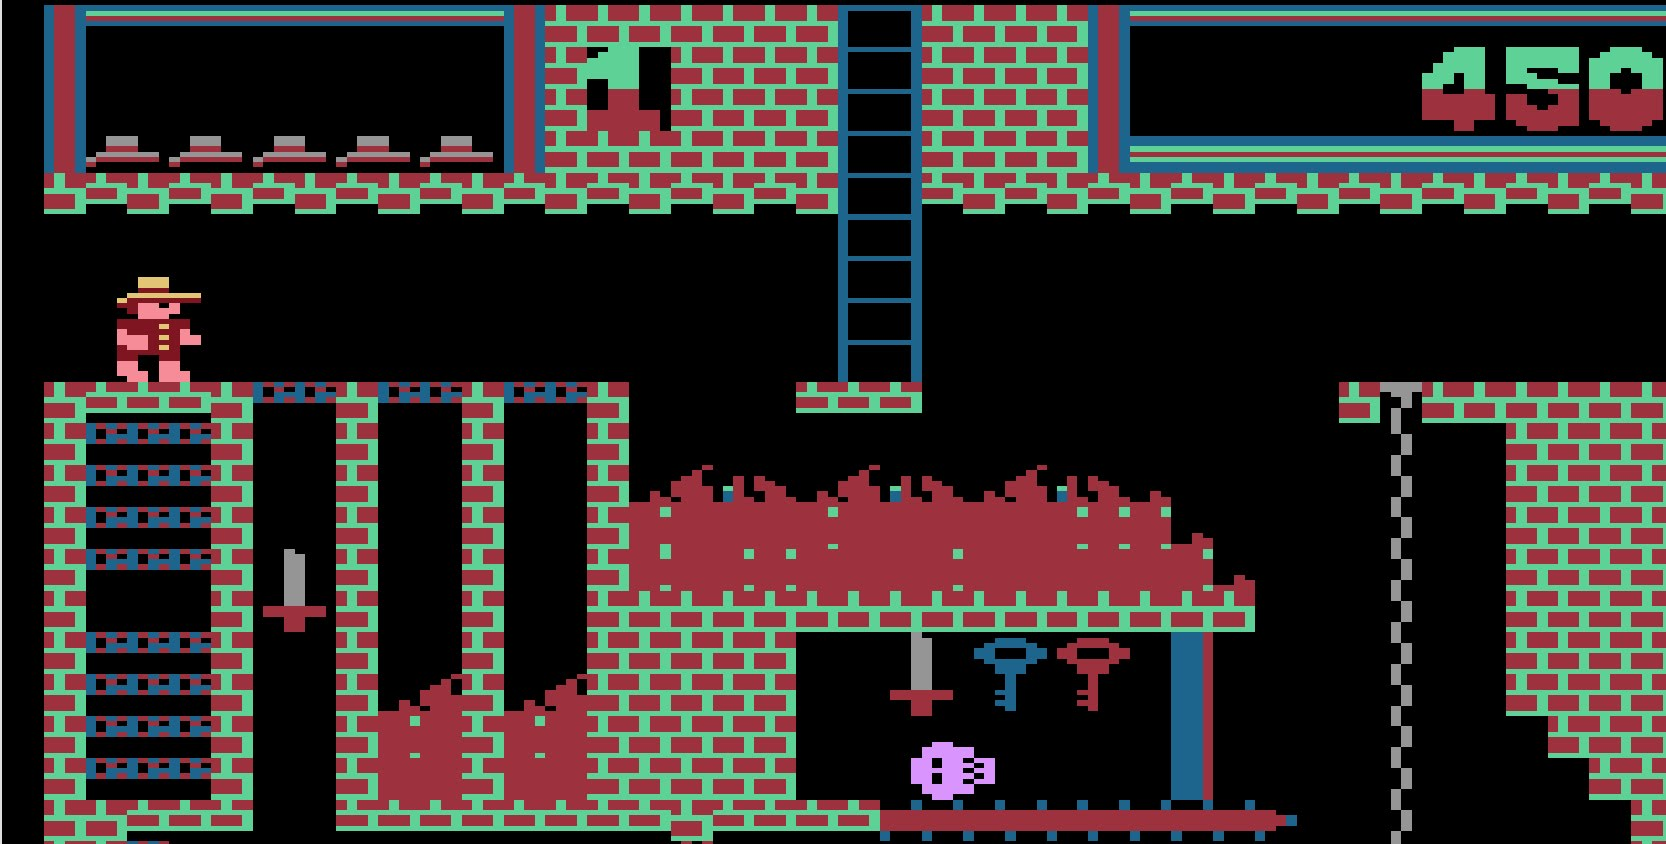
\includegraphics[width=1\linewidth]{images/monrev}
	\caption{Уровень игры Montezuma's Revenge}
	\label{fig:monrev}
\end{figure}


